% !TEX root = ../main.tex
%%--------------------------------------------------------------------------
%% SCENARIOS
%%--------------------------------------------------------------------------



\chapter{Use Cases}

This chapter is dedicated to explain the main use cases that can occur when using an application (in this case a web application) that takes advantage of the Pomasana API. Again, despite the following scenarios and use cases describe the interaction with an application and not directly with the system that is going to be developed, it is correct to assume that they reflect how the API are used; in fact all the functionalities of Pomasana are entirely exploitable through its API.

	\section{Actors}
	The only two possible type of actors are:
		
		\begin{description}

			\item[Unregistered User] He can only access the application Home Page and eventually register to Pomasana.

			\item[Registered User] He can exploit all the Pomasana functionalities.

		\end{description}

	\section{Use Cases}

		\subsection{Registration}

			\begin{description}

				\item[Actor] Unregistered User
			
				\item[Entry condition] None

				\item[Event Flow]\hfill

					\begin{itemize}

						\item The user opens the Home Page of Pomasana.

						\item The user is redirected to an Asana page that ask for permission.

						\item The system add the new user to the database.

						\item The system sends a confirmation email.

					\end{itemize}

				\item[Exceptions] If the user is not registered to Asana he is redirected to the Asana registration page.

				\item[Consequences] The user is registered to Pomasana and ready to use the system.

			\end{description}

		\subsection{Login}

			\begin{description}

				\item[Actor] Registered User
			
				\item[Entry condition] The user must be registered to Pomasana.

				\item[Event Flow]\hfill

					\begin{itemize}

						\item The user performs a login request on the Home Page.

						\item The system authenticates the user. 

						\item The user is redirected on the Todo Today page.

					\end{itemize}

				\item[Exceptions] If the user is not registered to Asana he is redirected to the Pomasana registration page.

				\item[Consequences] The user is now logged into the system and can use all its functionalities.

			\end{description}

		\subsection{Profile editing}

			\begin{description}

				\item[Actor] Registered User
			
				\item[Entry condition] The user must be logged into the system.

				\item[Event Flow]\hfill

					\begin{itemize}

						\item The user access his personal page.

						\item He modify the personal info and confirm.

						\item The system update the database with the new data.

					\end{itemize}

				\item[Exceptions] The new data are not complete and the system notify the error.

				\item[Consequences] The personal infos of the user are changed.

			\end{description}

		\subsection{Pomotask creation}

			\begin{description}

				\item[Actor] Registered User
			
				\item[Entry condition] The user must be logged into the system.

				\item[Event Flow]\hfill

					\begin{itemize}

						\item The user chooses an Asana project from a list.

						\item He select one task from the choosen project.

						\item The system updates the database with the new Pomotask data.

					\end{itemize}

				\item[Exceptions] The new data are not complete or correct and the system notify the error.

				\item[Consequences] There is a new Pomotask in the user Todo Today list.

			\end{description}

		\subsection{Pomotask editing}

			\begin{description}

				\item[Actor] Registered User
			
				\item[Entry condition] The user must be logged into the system.

				\item[Event Flow]\hfill

					\begin{itemize}

						\item The user choose a Pomotask from its Todo Today list.

						\item He modify the Pomotask info like the name or the estimate.

						\item He confirms the changes. 

						\item The system updates the database with the new Pomotask data.

					\end{itemize}

				\item[Exceptions] The new data are not complete or correct and the system notify the error.

				\item[Consequences] The info of the Pomotask are now updated.

			\end{description}

		\subsection{Pomotask deletion}

			\begin{description}

				\item[Actor] Registered User
			
				\item[Entry condition] The user must be logged into the system.

				\item[Event Flow]\hfill

					\begin{itemize}

						\item The user choose a Pomotask from its Todo Today list.

						\item He confirm the deletion.

						\item The system delete the Pomotask, leaving the corrispondent Asana task untouched.

					\end{itemize}

				\item[Exceptions]

				\item[Consequences] The Pomotask is now deleted from the database.

			\end{description}

		\subsection{Pomodoro addition}

			\begin{description}

				\item[Actor] Registered User
			
				\item[Entry condition] The user must be logged into the system.

				\item[Event Flow]\hfill

					\begin{itemize}

						\item The user choose a Pomotask from its Todo Today list.

						\item He adds the info of the new Pomodoro, like interruptions or notes.

						\item He confirms the info.

						\item The system updates the database with the new Pomdoro data.

						\item The system adds the Pomodoro to the associated Pomotask.

					\end{itemize}

				\item[Exceptions] The new data are not complete or correct and the system notify the error.

				\item[Consequences] The new Pomodoro is now persisted in the database.

			\end{description}


	\section{Use Case Diagram}

	Here we group all the use cases in a ``Use Case Diagram'' that helps to understands the dependencies between them.\\


		\begin{figure}[h!]
		  \centering
		    \centering{%
		      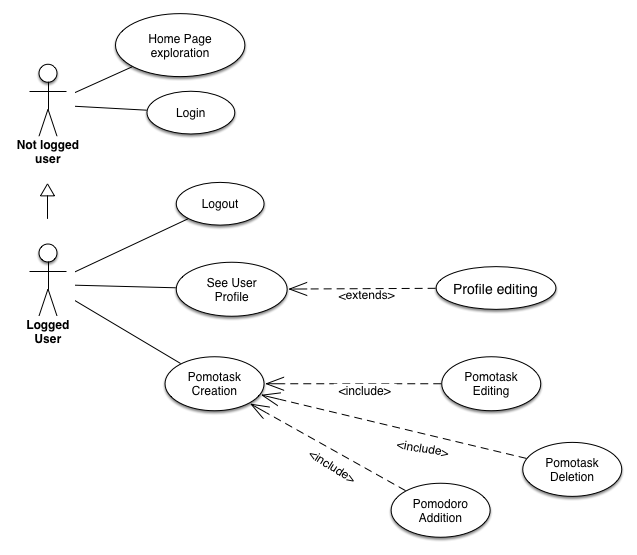
\includegraphics[width=1\textwidth]{use_case.png}}
		  \caption{Use Case Diagram}
		\end{figure}

	
